\icode{E-MI-CA-L3-261109-001}
在粗糙水平地面上放置一个边长为\(a\)、质量为\(M\)的正方体\(ABCD\)，正方体与地面间的动摩擦因数为\(\mu\)，在正方体右侧有一竖直光滑墙壁，如图所示，在墙壁和正方体之间放置一半径为\(R\)、质量为\(m\)的球，球的球心为\(O\)，\(OB\)与竖直方向的夹角为\(\theta\)，正方体和球均保持静止，重力加速度为\(g\)，最大静摩擦力等于滑动摩擦力。
\begin{enumerate}
	\item 求竖直墙壁对球的弹力大小；
	\item 若保持球的半径不变，只增大球的质量，为了不让正方体出现滑动，则球的质量最大值为多少。
\end{enumerate}
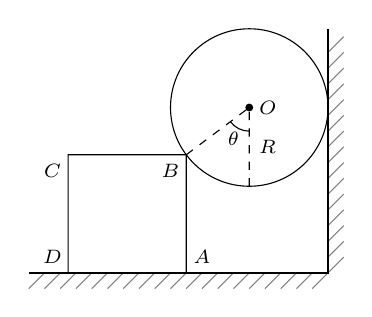
\begin{tikzpicture}[font=\scriptsize]
	\draw (0,0) rectangle(1.5,1.5) (2.3,2.1) circle(1);
	\draw[dashed] (1.5,1.5)--(2.3,2.1)--node[right]{\(R\)}(2.3,1.1);
		\fill (2.3,2.1)node[right]{\(O\)} circle(.05);
		\draw (2.3,1.8) arc(-90:-143:.3);
		\foreach \x in {-.5,-.3,...,3.1}
			\draw[gray] (\x,-.2)--++(.2,.2);
		\foreach \y in {0,.2,...,2.9}
			\draw[gray] (3.3,\y)--++(.2,.2);
		\draw[thick] (-.5,0)--(3.3,0)--(3.3,3.1);
		\node at(1.3,1.3){\(B\)};
		\node at(1.7,.2){\(A\)};
		\node at(-.2,1.3){\(C\)};
		\node at(-.2,.2){\(D\)};
		\node at(2.1,1.7){\(\theta\)};
	\end{tikzpicture}
\end{proset}
\begin{answer}
	\begin{enumerate}
		\item[(1)]\(F = \dfrac{Mg}{\cos\theta}\)
		\item[(2)]\(m = \dfrac{M}{2}\)
	\end{enumerate}
\end{answer}